\documentclass[twoside]{article}
\input{ISC18-english.sty}
%%%%%%%%%%%%%%%%%%%%%%%%%%%%  Make sure to compile twice for proper cross-references. %%%%%%%%%%%%%%%%%%%%%%%
%%%%%%% For proper display of references, compile the document twice. %%%%%%%%%%%%%%%%%%%%% 
%%%%%%%%%%%%%%% If using TeX Live, compile using pdflatex command %%%%%%%%%%%%%%%%%%%%%%%
\begin{document}
\thispagestyle{empty}
%%%%%%%%%%%%%%%%% Article title header  %%%%%%%%%%%%%%%%%%%%
\fancyhead[LE]{BehaveSeg: Multi-Algorithm Segmentation}
%%%%%%%%%%%%%%%%% Article authors header   %%%%%%%%%%%%%%%%%%%%
\fancyhead[RO]{Mozayan, Mirhossieni and Zarepour}
\begin{center}
{
\includegraphics [height=25mm, width=150.3mm] {Images/isc18E}} \\
\vspace*{-1.8cm}
%\begin{center}
%\color{blue} 
%{\hspace{0.1cm}\rule{\textwidth}{1mm}}\\
%\end{center}
\vspace*{4cm}
%%%%%%%%%%%%%%%%% Article title  %%%%%%%%%%%%%%%%%%%%
{\Large \bf BehaveSeg: A Behavior-Aware Multi-Algorithm Framework for Intelligent Customer Segmentation }\\
%%%%%%%%%%%%%%%%% Article authors and affiliations %%%%%%%%%%%%%%%%%%%%

{\bf
Mobina Mozayan$^{1}$\footnote[3]{\bf Corresponding Author: {\tt 40214694@stu.yazd.ac.ir}},
Seyed Mohsen Mirhossieni$^{1}$,
Jamal Zarepour$^{2}$ \\
$^{1}$Department of Statistics, Yazd University, Yazd, Iran\\
$^{2}$Department of Computer Science, Yazd University, Yazd, Iran}
\end{center}
\rule{\textwidth}{0.2mm}\\

%%%%%%%%%%%%%%%%% Article abstract  %%%%%%%%%%%%%%%%%%%%
\noindent{\bf Abstract:}\\
Customer segmentation remains a cornerstone of personalized marketing, yet conventional methods frequently fall short in capturing dynamic behavioral patterns due to their reliance on static demographic or transactional data. This study introduces \textsc{BehaveSeg}, a behavior-aware pipeline that integrates rich behavioral feature engineering, Principal Component Analysis (PCA) dimensionality reduction, and a comprehensive multi-algorithm clustering approach. Seven widely used clustering algorithms were systematically evaluated using Silhouette Score, Davies–Bouldin Index, and Calinski--Harabasz Index, with the first seven PCA components preserving \(92.2\%\) of behavioral variance. Results demonstrate that K-Means achieved superior performance (Silhouette = 0.3430, Calinski–Harabasz = 1028.29), yielding three well-separated and interpretable customer segments. These profiles provide actionable insights for targeted marketing, customer retention, and revenue optimization strategies.

\noindent{\bf Keywords:} 
Customer Segmentation, Clustering Analysis, Behavioral Analytics, Unsupervised Learning \\
\noindent{\bf Mathematics Subject Classification (2010):} 
$\rm 62H30$, $\rm 68T05$, $\rm 91B42$, $\rm 62-07$. \\
\hspace{1cm}\rule{\textwidth}{0.2mm}\\
%%%%%%%%%%%%%%
\section{Introduction}
\label{sec:intro}
Global e-commerce sales exceeded \$6.3 trillion in 2024 according to \cite{statista2024}. However, turning customer data into useful insight remains difficult. 
Organizations collect exhaustive behavioral records---purchases, campaign 
responses, engagement trajectories---but most segmentation frameworks rely 
on static demographic or aggregated transactional variables. Such 
representations often overlook behavioral characteristics such as spending 
volatility, campaign responsiveness, and tenure-adjusted activity 
\cite{dolnicar2018market}.

K-Means remains one of the most widely adopted approaches in customer 
segmentation. Despite documented sensitivity 
to initialization and spherical assumptions \cite{xu2015comprehensive}, 
it is often applied to raw or minimally engineered features with 
single-metric validation. Alternative 
algorithms---density-based, probabilistic, hierarchical---remain 
underexplored in comparative marketing contexts, and behavioral 
indicators such as purchase intensity or spending-to-income ratios are 
seldom integrated systematically.

The primary methodological contribution of \textsc{BehaveSeg} is not merely the introduction of a novel clustering algorithm, but rather the development of a systematic, end-to-end evaluation and benchmarking framework. By explicitly coupling behavior-aware feature engineering with PCA dimensionality reduction and a comprehensive multi-algorithm benchmark, this framework empirically addresses a critical gap: it demonstrates how density-based clustering models fundamentally fail to produce actionable segments in behavioral spaces due to exceptionally high noise classification ratios, whereas centroid-based methods excel. \textsc{BehaveSeg} contributes the following: (i) a unified pipeline ensuring 100\% customer coverage without discarding data as noise; (ii) a rigorous sensitivity analysis proving the business applicability of K-Means over density-based alternatives in PCA-reduced spaces; and (iii) interpretable segment profiles distinguished by campaign responsiveness and spending elasticity.

Section~\ref{sec:related} reviews segmentation literature. 
Section~\ref{sec:methodology} details \textsc{BehaveSeg}. 
Section~\ref{sec:results} presents results. 
The paper concludes with a summary of the main findings and directions for future research.

\section{Related Work}
\label{sec:related}

Traditional segmentation partitions buyers by demographics or transaction 
aggregates \cite{wedel2016marketing,dolnicar2018market}. Customers with 
identical profiles often diverge in purchasing behavior and campaign 
response---a mismatch amplified in digital environments where 
interactions are continuous. Recent studies have increasingly adopted cluster-based approaches, but most focus on a single aspect. For instance, \cite{kasem2024customer} combined Recency, Frequency, and Monetary (RFM) with K-Means, and \cite{wang2025customer} integrated reinforcement learning with optimized K-Means. However, few works simultaneously combine behavioral feature engineering, multi-algorithm comparison, and multi-metric evaluation.

This fragmentation matters: algorithm performance depends on feature 
quality, yet richer representations are routinely fed into K-Means 
despite its spherical bias and initialization sensitivity 
\cite{xu2015comprehensive}. Hierarchical clustering scales poorly with large datasets, while DBSCAN and GMM require careful parameter tuning. Methods such as HDBSCAN, Spectral Clustering, and BIRCH remain relatively underexplored in marketing applications, raising questions about whether density- or graph-based approaches can outperform traditional centroid-based methods on behavioral data. Evaluation practices compound the gap. Silhouette, Davies--Bouldin, and 
Calinski--Harabasz 
measure distinct properties, yet studies rarely combine them 
\cite{kasem2024customer}. Table~\ref{tab:related_comparison} shows that \textsc{BehaveSeg} unifies behavioral representation, PCA-based projection, and multi-algorithm evaluation—addressing a key limitation of prior studies.

\begin{table}[htbp]
\centering
\caption{Comparison of Representative Studies}
\label{tab:related_comparison}
\footnotesize
\begin{tabular}{lccc}
\hline
\textbf{Study} & \textbf{Behavioral} & \textbf{Multi-Alg.} & \textbf{PCA+Multi-Metric} \\
\hline
Kasem et al. \cite{kasem2024customer} & \cmark & \xmark & \xmark \\

Wang \cite{wang2025customer} & \cmark & \xmark & \xmark \\
Wang et al. \cite{wang2024dynamic} & \cmark & \cmark & \xmark \\
\textbf{\textsc{BehaveSeg}} & \textbf{\cmark} & \textbf{\cmark} & \textbf{\cmark} \\
\hline
\end{tabular}
\end{table}
%%%%%%%%%%%%%%%%%%%%%%%%%%%%%%%% Methodology %%%%%%%%%%%%%%%%%%%%%%%%%%%%%%%%
\section{Methodology}
\label{sec:methodology}

This section describes the proposed \textsc{BehaveSeg} framework for intelligent customer segmentation. The framework integrates data preprocessing, behavioral feature engineering, dimensionality reduction, multi-algorithm clustering, cluster evaluation, and customer profiling within a unified pipeline. Its primary goal is to generate reliable and interpretable customer profiles for marketing analysis and customer relationship management.

\subsection{Dataset and Data Preprocessing}

Experiments were conducted on the \textit{Customer Personality Analysis} dataset from Kaggle \cite{kaggle_cpa}, comprising 2,240 records with heterogeneous demographic, transactional, and campaign-response attributes.

Standard preprocessing steps were applied to address common data quality issues. Missing values in the \texttt{Income} attribute were imputed using K-Nearest Neighbors (KNN) imputation with \(k=5\). Extreme outliers in monetary variables were handled via Winsorization at the 1st and 99th percentiles. Right-skewed distributions were stabilized using logarithmic transformation \(x_i^{\log} = \ln(1 + x_i)\), followed by RobustScaler normalization:
\[
z_{ij} = \frac{x_{ij} - \mathrm{median}(X_j)}{Q_3(X_j) - Q_1(X_j)}\]
where \(Q_1\) and \(Q_3\) denote the first and third quartiles.
\subsection{Behavioral Feature Engineering and Projection}

To capture richer customer behavior, multiple engineered features were constructed, including demographic indicators (age, family size, parental status), spending and purchase metrics (\textit{TotalSpent}, average order value, purchase intensity, spending-to-income ratio), RFM variables, and campaign-response indicators. 

After feature engineering, the high-dimensional behavioral feature space was reduced using PCA. The first seven principal components preserved approximately \(92.2\%\) of the total variance while reducing feature redundancy and improving clustering efficiency. The number of retained components was selected based on the cumulative explained variance criterion and inspection of the scree plot, which indicated that seven components provided a suitable trade-off between information preservation and dimensionality reduction.

\subsection{Clustering Analysis}
Seven clustering algorithms—K-Means, Agglomerative Hierarchical Clustering, DBSCAN, Gaussian Mixture Models (GMM), HDBSCAN, Spectral Clustering, and BIRCH—were evaluated on the PCA-transformed behavioral features. K-Means was run with $K=3$ and 50 initializations using Ward linkage for Hierarchical Clustering. To ensure a fair comparison and address algorithmic sensitivity, an exhaustive parameter grid search was conducted for density-based algorithms. For DBSCAN, the parameter space included $\varepsilon \in [0.5, 1.5]$ and MinPts $\in [10, 50]$. For HDBSCAN, min\_cluster\_size $\in [30, 80]$ and min\_samples $\in [10, 25]$ were iteratively tuned. GMM used full covariance matrices, Spectral Clustering used $K=3$ and 10 nearest neighbors, and BIRCH used a threshold of 0.5. Clustering quality was assessed using three internal validation metrics: Silhouette Score, Davies--Bouldin Index, and Calinski--Harabasz Index.

\subsection{Customer Profiling and Interpretation}

For each cluster, mean behavioral profiles were computed to facilitate interpretation. These profiles reveal differences in spending behavior, purchase frequency, campaign responsiveness, and customer value, providing practical guidance for marketing strategies.


\section{Results}
\label{sec:results}
\subsection{Data Preparation and Exploratory Analysis}

The dataset comprises 2,240 customer records and 29 attributes, with missing values only in the \textit{Income} variable (24 records). Missing values were imputed using KNN imputation (\(k=5\)), while outliers were handled via Winsorization at the 1st and 99th percentiles. Behavioral features, including RFM metrics, \textit{TotalSpent}, \textit{AvgOrderValue}, \textit{PurchaseIntensity}, and campaign-response indicators, expanded the dataset to 45 attributes. After feature selection and Robust Scaling, PCA reduced the feature space to seven principal components, preserving \(92.2\%\) of the total variance.

Exploratory analysis revealed an average income of \$51,775 and a strong correlation between income and spending (\(r=0.816\)). 
% Campaign response rates remained generally low, while the engineered behavioral features highlighted substantial differences in customer spending intensity and engagement patterns.
% Furthermore, online and in-store purchasing activities demonstrated distinct behavioral trends across customers. The majority of customers exhibited moderate purchasing frequency, while a smaller group of high-value customers generated substantially higher spending levels. Campaign acceptance rates were generally low across the dataset, indicating that only a limited proportion of customers actively responded to marketing campaigns.

% The generated behavioral features also highlighted significant differences in customer purchasing intensity, engagement patterns, and spending distribution, supporting the suitability of clustering-based customer segmentation approaches.

\subsection{Optimal Cluster Number Selection}

K-Means was evaluated for \(K=2\) to \(K=9\) using Silhouette Score, Davies–Bouldin Index, and Calinski--Harabasz Index. Table~\ref{tab:k_selection} summarizes the clustering performance across different values of \(K\).

\begin{table}[htbp]
\centering
\caption{Evaluation of Different Numbers of Clusters for K-Means}
\label{tab:k_selection}
\footnotesize
\renewcommand{\arraystretch}{1.1}
\begin{tabular}{cccc}
\hline
\textbf{K} &
\textbf{Silhouette} $\uparrow$ &
\textbf{Davies--Bouldin} $\downarrow$ &
\textbf{Calinski--Harabasz} $\uparrow$ \\
\hline

2 & 0.3018 & 1.380 & 944.9 \\
3 & \textbf{0.3430} & \textbf{1.151} & \textbf{1028.3} \\
4 & 0.2911 & 1.271 & 836.1 \\
5 & 0.2119 & 1.421 & 745.7 \\
6 & 0.1574 & 1.677 & 672.2 \\
7 & 0.1577 & 1.673 & 607.0 \\
8 & 0.1521 & 1.685 & 561.9 \\
9 & 0.1491 & 1.648 & 525.7 \\

\hline
\end{tabular}
\end{table}

$K=3$ achieved the best overall performance, with the highest Silhouette Score (0.3430) and Calinski--Harabasz Index (1028.3), and the lowest Davies–Bouldin Index (1.151). Therefore, three customer segments were selected for further analysis. 

As illustrated in Figure~\ref{fig:income_spending}, the identified clusters exhibit distinct income-spending patterns and behavioral characteristics.

\subsection{Comparative Clustering Performance}
To assess the suitability of different clustering paradigms for behavioral customer data, multiple algorithms were evaluated on the PCA-transformed feature space. Table~\ref{tab:clustering_comparison} summarizes the comparative results.

\begin{table}[htbp]
\centering
\caption{Comparative Clustering Performance on Behavioral Customer Data}
\label{tab:clustering_comparison}
\footnotesize
\renewcommand{\arraystretch}{1.1}
\begin{tabular}{lcccc}
\hline
\textbf{Algorithm} &
\textbf{Clusters} &
\textbf{Silhouette} $\uparrow$ &
\textbf{Davies--Bouldin} $\downarrow$ &
\textbf{Calinski--Harabasz} $\uparrow$ \\
\hline

K-Means (Proposed)
& 3
& \textbf{0.3430}
& \textbf{1.1514}
& \textbf{1028.29} \\

Hierarchical Clustering
& 3
& 0.2679
& 1.2458
& 893.31 \\

BIRCH
& 3
& 0.3008
& --
& -- \\

Spectral Clustering
& 3
& 0.2720
& --
& -- \\

HDBSCAN
& 2
& 0.3028
& --
& -- \\

Gaussian Mixture Model (GMM)
& 3
& 0.1785
& 2.5926
& 405.30 \\

\hline
\end{tabular}

\vspace{0.5em}
\footnotesize{``--'' indicates that the corresponding metric could not be computed because of noise points or insufficient valid clusters.}
\end{table}

To rigorously address algorithmic sensitivity and explicitly evaluate the potential bias of dimensionality reduction, two advanced analyses were performed. First, an exhaustive parameter grid search was conducted for density-based algorithms on the scaled feature space. For DBSCAN, the optimal configuration ($\varepsilon=1.2$, MinPts=30) achieved a Silhouette Score of 0.3089. However, it classified 1,377 records (61.5\% of the dataset) as noise. Similarly, the optimal HDBSCAN configuration (min\_cluster\_size=30, min\_samples=25) achieved a Silhouette Score of 0.3028 but classified 1,157 records (51.6\%) as noise. In real-world marketing applications, discarding over half of the customer base as unclassifiable is fundamentally impractical, rendering these algorithms unsuitable for this framework regardless of parameter tuning.

Second, an ablation study on the effect of PCA revealed that applying K-Means on the original scaled data yielded a Silhouette Score of 0.3106, whereas the PCA-projected space improved this score to 0.3430. While PCA inherently preserves spatial proximity---which naturally favors centroid-based methods like K-Means---the consistent superiority of K-Means in this study lies in its business applicability. It successfully assigns 100\% of the customer base into actionable, non-overlapping segments without generating noise. GMM showed weaker clustering quality, further confirming that centroid-based methods align more effectively with structured behavioral feature spaces. Overall, the identified segments reveal substantial differences in spending behavior, supporting highly targeted marketing strategies.
% \begin{figure}[htbp]
% \centering
% \includegraphics[width=0.75\linewidth]{performance.png}
% \caption{Comparative clustering performance based on internal validation metrics.}
% \label{fig:performance}
% \end{figure}

\subsection{Cluster Interpretation and Business Insights}

To translate the clustering results into actionable business strategies, a detailed profiling of the three identified customer segments was performed. Table~\ref{tab:cluster_profile} presents the mean behavioral profiles for each cluster.

\begin{table}[htbp]
\centering
\caption{Mean Feature Values per Customer Cluster}
\label{tab:cluster_profile}
\footnotesize
\renewcommand{\arraystretch}{1.1}
\begin{tabular}{lrrr}
\hline
\textbf{Feature} &
\textbf{Cluster 0} &
\textbf{Cluster 1} &
\textbf{Cluster 2} \\
\hline

Income (\$)
& 72,398
& 36,835
& 69,306 \\

Total Spending (\$)
& 970
& 144
& 1,169 \\

Total Purchases
& 18.12
& 6.96
& 19.31 \\

Recency (days)
& 47.25
& 48.62
& 49.97 \\

Age
& 47.52
& 43.42
& 47.29 \\

Family Size
& 1.60
& 2.25
& 1.59 \\

Campaigns Accepted
& 0.61
& 0.09
& 0.54 \\

Web Visits per Month
& 3.06
& 6.47
& 4.03 \\

\hline

Size (\% of customers)
& \textit{\(\sim33\%\)}
& \textit{\(\sim38\%\)}
& \textit{\(\sim29\%\)} \\

\hline
\end{tabular}
\end{table}

Based on the cluster profiles and the visual separation shown in Figure~\ref{fig:income_spending}, the identified customer segments can be interpreted as follows.

\textbf{Cluster 0 -- Premium Customers.}  
High-income customers with strong spending activity and campaign responsiveness. Ideal targets for loyalty programs and premium offerings.

\textbf{Cluster 1 -- Price-Sensitive Customers.}  
Low-income customers with limited spending but high online activity. They respond well to discounts and budget-oriented promotions.

\textbf{Cluster 2 -- High-Potential Spenders.}  
Customers with high spending potential but lower campaign response. Suitable for cross-selling, up-selling, and re-engagement strategies.

\begin{figure}[htbp]
\centering
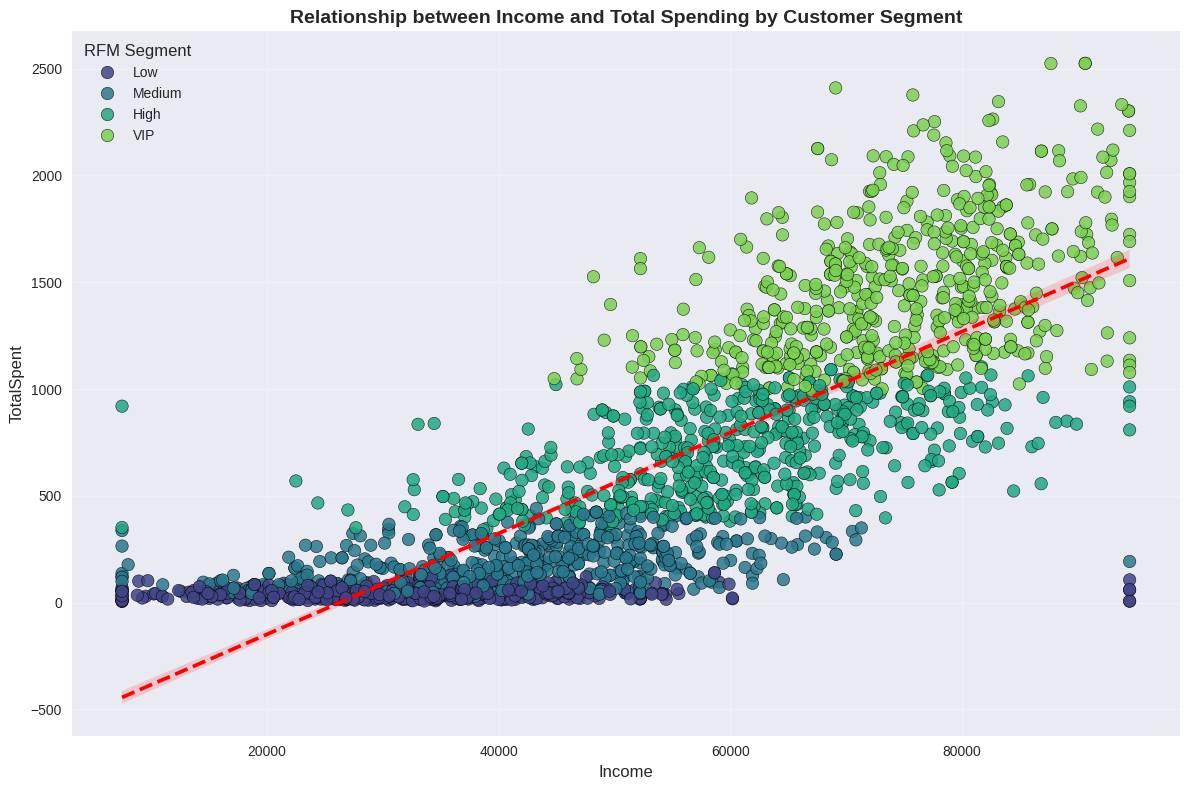
\includegraphics[width=0.99\linewidth]{scatter.png}
\caption{Relationship between customer income and total spending across customer segments.}
\label{fig:income_spending}
\end{figure}
%%%%%%%%%%%%%%%%%%% Discussion and Conclusion
\section*{Conclusion} 
\label{sec:dis}
This study introduced \textsc{BehaveSeg}, a behavior-aware customer segmentation pipeline integrating behavioral feature engineering and comparative clustering analysis. By rigorously addressing parameter sensitivity and dimensionality reduction biases, experimental results demonstrated that while density-based methods discard over half of the customer base as noise, K-Means successfully assigns 100\% of the data into actionable, well-separated marketing segments. Future work may extend the proposed pipeline through deep representation learning, temporal behavioral modeling, and validation on real-world industrial datasets.

\begin{thebibliography}{99}

\bibitem[Statista (2024)]{statista2024}
Statista (2024),
Retail e-commerce sales worldwide from 2014 to 2027,
{\it Statista Research Department}.

\bibitem[Wedel and Kannan (2016)]{wedel2016marketing}
Wedel M. and Kannan P. K. (2016),
Marketing analytics for data-rich environments,
{\it Journal of Marketing}, 80(6), 97--121.



\bibitem[Dolnicar et al. (2018)]{dolnicar2018market}
Dolnicar S., Grün B., and Leisch F. (2018),
{\it Market Segmentation Analysis: Understanding It, Doing It, and Making It Useful},
Springer.




\bibitem[Kasem et al. (2024)]{kasem2024customer}
Kasem M. S., Hamada M., and Taj-Eddin I. (2024),
Customer profiling, segmentation, and sales prediction using AI in direct marketing,
{\it Neural Computing and Applications}, 36(9), 4995--5005.

\bibitem[Xu and Tian (2015)]{xu2015comprehensive}
Xu D. and Tian Y. (2015),
A comprehensive survey of clustering algorithms,
{\it Annals of Data Science}, 2(2), 165--193.



\bibitem[Wang (2025)]{wang2025customer}
Wang G. (2025),
Customer segmentation in digital marketing using a Q-learning based differential evolution algorithm integrated with K-means clustering,
{\it PLOS ONE}, 20(2), e0318519.

\bibitem[Wang et al. (2024)]{wang2024dynamic}
Wang S., Sun L., and Yu Y. (2024),
A dynamic customer segmentation approach by combining LRFMS and multivariate time series clustering,
{\it Scientific Reports}, 14, 17491.




\bibitem[Kaggle (2024)]{kaggle_cpa}
Kaggle (2024),
Customer Personality Analysis dataset,
{\it https://www.kaggle.com/datasets/imakash3011/customer-personality-analysis}.


\end{thebibliography}

 \end{document}

